\documentclass[12pt]{article}
\usepackage[top=1in, bottom=1in, left=.75in, right=.75in]{geometry}
\usepackage{amsmath, enumerate}
\usepackage{fancyhdr}
\usepackage{graphicx, xcolor, setspace}
\usepackage{txfonts}
\usepackage{multicol,coordsys,pgfplots}
\usepackage[scaled=0.86]{helvet}
\renewcommand{\emph}[1]{\textsf{\textbf{#1}}}
\usepackage{anyfontsize}
% \usepackage{times}
% \usepackage[lf]{MinionPro}
\usepackage{tikz,pgfplots}
%\def\degC{{}^\circ{\rm C}}
\def\ra{\rightarrow}
\usetikzlibrary{calc,arrows.meta}
\pgfplotsset{compat = newest}
\newcommand{\blank}[1]{\rule{#1}{0.75pt}}

\pgfplotsset{my style/.append style={axis x line=middle, axis y line=
middle, xlabel={$x$}, ylabel={$y$}}}

%axis equal

%yticklabels={,,} , xticklabels={,,}

% \setmainfont{Times}
% \def\sansfont{Lucida Grande Bold}
\parindent 0pt
\parskip 4pt
\pagestyle{fancy}
\fancyfoot[C]{\emph{\thepage}}
\fancyfoot[R]{v1} %%%%%% <-- Version Info
\fancyhead[L]{\ifnum \value{page} > 1\relax\emph{Math F251X: Midterm 1}\fi}
\fancyhead[R]{\ifnum \value{page} > 1\relax\emph{Fall 2024}\fi}
\headheight 15pt
\renewcommand{\headrulewidth}{0pt}
\renewcommand{\footrulewidth}{0pt}
\let\ds\displaystyle
\def\continued{{\emph {Continued....}}}
\def\continuing{{\emph {Problem \arabic{probcount} continued....}}\par\vskip 4pt}


\newcounter{probcount}
\newcounter{subprobcount}
\newcommand{\thesubproblem}{\emph{\alph{subprobcount}.}}
\def\problem#1{\setcounter{subprobcount}{0}%
\addtocounter{probcount}{1}{\emph{\arabic{probcount}.\hskip 1em(#1)}}\par}
\def\subproblem#1{\par\hangindent=1em\hangafter=0{%
\addtocounter{subprobcount}{1}\thesubproblem\emph{#1}\hskip 1em}}
\def\probskip{\vskip 10pt}
\def\medprobskip{\vskip 2in}
\def\subprobskip{\vskip 45pt}
\def\bigprobskip{\vskip 4in}


\newenvironment{subproblems}{%
\begin{enumerate}%
\setcounter{enumi}{\value{subprobcount}}%
\renewcommand{\theenumi}{\emph{\alph{enumi}}}}%
{\setcounter{subprobcount}{\value{enumi}}\end{enumerate}}


\newcommand{\be}{\begin{enumerate}}
\newcommand{\ee}{\end{enumerate}}


\begin{document}
{\emph{\fontsize{26}{28}\selectfont Fall 2024 \hfill
%{\fontsize{32}{36}\selectfont Calculus 1: Midterm 1}
\hfill Math F251X}}

\begin{center}
{\emph{%\fontsize{26}{28}\selectfont Spring 2024 
%%\hfill
{\fontsize{32}{36}\selectfont Calculus 1: Midterm 1}
%%\hfill Math F251X}
}}
\end{center}

%\vskip 2cm
\strut\vtop{\halign{\emph#\hskip 0.5em\hfil&#\hbox to 2in{\hrulefill}\cr
\emph{\fontsize{18}{22}\selectfont Name:}&\cr
%\noalign{\vskip 10pt}
%\emph{\fontsize{18}{22}\selectfont Student Id:}&\cr
%\noalign{\vskip 10pt}
%\emph{\fontsize{18}{22}\selectfont Calculator Model:}&\cr
}}
\hfill
\vtop{\halign{\emph{\fontsize{18}{22}\selectfont #}\hfil& \emph{\fontsize{18}{22}\selectfont\hskip 0.5ex $\square$ #}\hfil\cr
Section: & 9:15am (James Gossell)\cr
\noalign{\vskip 4pt}
         & 11:45am (Jill Faudree)\cr
\noalign{\vskip 4pt}
         & 11:45am (Leah Berman)\cr
\noalign{\vskip 4pt}
         & async (James Gossell)\cr}}

\vfill
{\fontsize{18}{22}\selectfont\emph{Rules:}}

\begin{itemize}
\item Partial credit will be awarded, but you must show your work.

\item You may have a single handwritten $3'' \times 5''$ notecard, both sides.

\item Calculators are {\bf not} allowed. 

\item Place a box around your  \fbox{FINAL ANSWER} to each question where appropriate.

\item Turn off anything that might go beep during the exam.

\end{itemize}

%If you need extra space, you can use the back sides of the pages.
%Please make it obvious  when you have done so.



Good luck!
\vfill
\def\emptybox{\hbox to 2em{\vrule height 16pt depth 8pt width 0pt\hfil}}
\def\tline{\noalign{\hrule}}
\centerline{\vbox{\offinterlineskip
{
\bf\sf\fontsize{18pt}{22pt}\selectfont
\hrule
\halign{
\vrule#&\strut\quad\hfil#\hfil\quad&\vrule#&\quad\hfil#\hfil\quad
&\vrule#&\quad\hfil#\hfil\quad&\vrule#\cr
height 3pt&\omit&&\omit&&\omit&\cr
&Problem&&Possible&&Score&\cr\tline
height 3pt&\omit&&\omit&&\omit&\cr
&1&&14&&\emptybox&\cr\tline
&2&&15&&\emptybox&\cr\tline
&3&&10&&\emptybox&\cr\tline
&4&&15&&\emptybox&\cr\tline
&5&&8&&\emptybox&\cr\tline
&6&&12&&\emptybox&\cr\tline
&7&&6&&\emptybox&\cr\tline
&8&&8&&\emptybox&\cr\tline
&9&&12&&\emptybox&\cr\tline \tline
&Extra Credit&&(5)&&\emptybox&\cr\tline
&Total&&100&&\emptybox&\cr
}\hrule}}}

\newpage
\problem{14 points} 

The graph of a function $g(x)$ is shown below. The domain of the function is $[-4,5]$.
Use the graph to answer each question below. If the limit is infinite, indicate that with $\infty$ or $-\infty.$ If the value does not exist or is undefined, write {\sf DNE}.\\

\newcommand{\ans}{\rule{1cm}{.5pt}}

\begin{center}
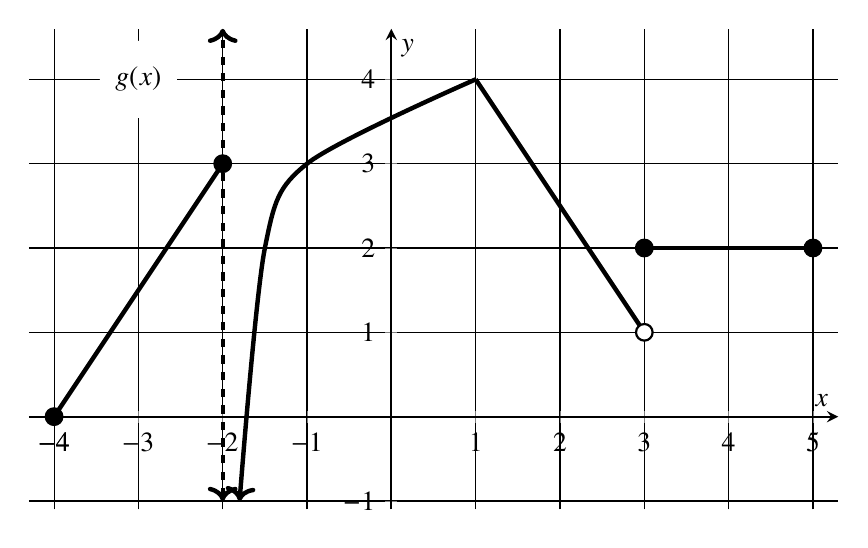
\begin{tikzpicture}[scale = 1]
\begin{axis}[scale=1.5, thick, my style, xtick={-4,-5,-4,...,5}, ytick={-1,1,2,...,4},
xmin=-4.3, xmax=5.3, ymin=-1.1, ymax=4.6, minor y tick num=0,
        minor x tick num=0, mark size=3.0pt, grid=both, grid style={ thin, black, %dashed
        }, axis equal image]
% %%asymptote
\addplot[dashed,<->, ultra thick] coordinates {(-2,-1) (-2,4.6)};      
%%points solid
\addplot[mark=*,only marks] coordinates {(-4,0)(-2,3)%(1,4)
(3,2)(5,2)};
%%points open
\addplot[mark=*,fill=white,only marks] coordinates {(3,1)};
%%Curves
\addplot[ultra thick] coordinates {(-4,0)(-2,3)};
\addplot[ultra thick] coordinates {(1,4)(3,1)};
\addplot[ultra thick] coordinates {(3,2)(5,2)};
%\addplot[<-,ultra thick, smooth, variable=\x, samples=100, domain=-3:-2.9] plot(\x,{1/(\x+2)^2 - 0.333});
\addplot[ultra thick, smooth, ->] coordinates {(1,4)(-1,3)(-1.5,2)%(-1.7,0.1)
(-1.8,-1)};
\node[fill=white,circle] at (-3,4)  {$g(x)$};
\end{axis}

\end{tikzpicture}
\end{center}

%\begin{enumerate}

\begin{subproblems}

\begingroup
%\color{blue} % Set the table color to blue

%\renewcommand{\baselinestretch}{3} % Adjust row height
%\linespread{3}

\setlength{\parskip}{2.5em}
\setlength{\columnsep}{1 cm}
\begin{multicols}{3}
\item $\ds{\lim_{ x\to-2^{-}}g(x)}$ = \ans

\item $\ds{\lim_{ x\to-2^{+}}g(x)}$ = \ans

%\item $\ds{\lim_{x\to-2}g(x)}$ = \ans


\item $g(1)$ = \ans
\columnbreak



\item $\ds{\lim_{ x\to1} g(x)}$ = \ans



\item $\ds{\lim_{ x\to1^{-}} g'(x)}$ = \ans \ \\[1ex]
 {\small {\it Note this is asking about the limit of the derivative.}}

\item $g'(1)$ = \ans

\columnbreak


\item $g'(2)$ = \ans

\item $\ds{\lim_{ x\to 3} g(x)}$ = \ans

\item $g'(4)$ = \ans

\end{multicols}

\endgroup

\bigskip

 \item List all \emph{$\mathbf{x}$-values} in the set $(-4, 5)$ where the function $g(x)$ is \emph{not} continuous.\\
 
 
$x = $ \ \hrulefill

\bigskip

\item Fill in the empty boxes to make a true sentence.

The function $g(x)$ has a vertical asymptote with equation \fbox{\rule{0pt}{2em}\hspace{2.5cm}} because
\[ \lim_{\fbox{\strut\hspace{1.5cm}}} g(x) = \fbox{\strut\hspace{1.5cm}}.\]

\end{subproblems}




\newpage


%%%%%% Compute the limits

\problem{15 points} Compute the following limits. Show your work. Use limit notation where necessary; you will be graded both on your computation and on your correct use of notation.

Give the most complete answer. Specifically, if the limit approaches $+ \infty$ or $- \infty$, write that. The answer DNE is insufficient in this case.
\begin{subproblems}
\item $\displaystyle \lim_{x \rightarrow 3} \frac{12-4x}{x^2-10x+21}$
%\textcolor{red}{5 pts}


	\vfill
	
	\item $\displaystyle \lim_{x \rightarrow 0} \frac{-2\cos x}{\sin x - 1}$
	%\textcolor{red}{3 pts}
	
	\vfill
	
	\item $\displaystyle \lim_{x \rightarrow 4^+} \frac{2
	x+17}{(x-4)(x-5)}$
	%\textcolor{red}{2 pts}
	\vfill
	
	\item  $\displaystyle \lim_{x \rightarrow 3} \displaystyle{\frac{\dfrac{x}{3}-\dfrac{3}{x}}{x-3}}$
	%\textcolor{red}{5 pts}
	\vfill

\end{subproblems}

\newpage

%%% Definition of the derivative
\problem{10 points}



 Consider the function
 \[\displaystyle f(x)=\sqrt{2-x}.\] 
Use the \emph{limit definition of the derivative} to compute the derivative, and show your work using all appropriate notation.  No credit will be awarded for using other methods.  You must write limits where necessary to receive full credit. 

The limit definition of the derivative:
\[ f'(x) = \lim_{h\to 0}\frac{f(x+h) - f(x)}{h}.\]

\vfill


\newpage

%Straight derivative problems
\problem{15 points} For each of the following functions, compute the derivative. 
\emph{You do not need to simplify your answers.} Your answer must begin with $f'(x)$ or similar notation, as appropriate to the problem.
 
\begin{subproblems}

	\item $\displaystyle{f(x)=x^{2.4}+\frac{\cos(x)}{5}+\frac{\sqrt[3]{x}}{3}+\sqrt{3}}$
	\vfill
	\item $\displaystyle{g(y)=y \sin(y)}$
	\vfill
	\item $\displaystyle{h(\theta)= \frac{\theta^4}{\theta^3+6}}$
	\vfill


\end{subproblems}

\newpage

%%% Function and derivative interpretation

\problem{8 points} 
Hopewell Cape, off the east coast of Canada, is known to have one of the highest tides in the world. The function $D(t)$ models the water depth at Hopewell Cape over a day, and is given by
\[D(t)=7+5 \cos\left(\:0.503(t-6.75)\:\right)\]
In this function, $D$ is water depth in meters and $t$ is measured in hours after midnight. \\

	\begin{subproblems}
	\item Explain the meaning of the fact that \fbox{$D(4)=7.9$} in the context of the problem. Make sure your explanation is one that a typical precalculus student could understand,  and don't forget to include units.
	\vfill
	\item Explain the meaning of the fact that \fbox{$D'(4)=2.5$} in the context of the problem. Make sure your explanation is one that a typical precalculus student could understand. (Do not use the word \emph{derivative}!) And don't forget to include units.
	\vfill
	\item Using the facts that \fbox{$D(4)=7.9$ and $D'(4)=2.5$}, estimate the water depth at 5:00 AM.
	%\textcolor{red}{To keep this or not? Replace with last part?}
	
	\vfill
	\item  Do you expect $D'(t)$ to ever take on negative values? Explain your answer. 
	\vfill
	\end{subproblems}
\newpage



%%%%%  tangent lines
\problem{12 points} Consider the function 
$\ds g(x) = \frac{1}{x}+8x^2 .$

\begin{subproblems}

 \item Find $g'(x)$. 
  (You do not need to use the limit definition of the derivative to answer this problem.)
  
\vfill

 \item Write an equation for the tangent line to $g(x)$ when $x=1.$   \\
 
 \vfill
  
 
  
  \item Determine the $x$-coordinates of all points on the graph of $g(x)$ where there is a \emph{horizontal} tangent line. Show your work.
  
  \vfill
  

\end{subproblems}

%%continuity
\problem{6 points} 
Consider the piecewise-defined function given below. The value $a$ is a constant whose value you do not yet know.

\[ f(x) = \begin{cases}
ax^{2} + 4 & \text{ if } x \geq 3\\
\frac{2}{x-1}& \text{ if }  x < 3
\end{cases}
\]
\begin{subproblems}

\item What should $a$ be so that $f(x)$ is continuous at $x = 3$? Justify your answer with limits, and show your work.

\vfill

\item  Identify any other points where $f(x)$ is not continuous. Explain how you know there is a discontinuity. Identify the type of discontinuity.

\vfill
\end{subproblems}


\newpage

%%%%SKETCH DERIVATIVE FROM GRAPH OF FUNCTION

\problem{8 points} 
The graph of a function $k(x)$ is shown below. On the set of axes below the graph, sketch the derivative, $k'(x)$. 

Indicate any asymptotes the derivative might have using dashed lines, and indicate any points where the derivative is undefined using open circles.
\begin{center}
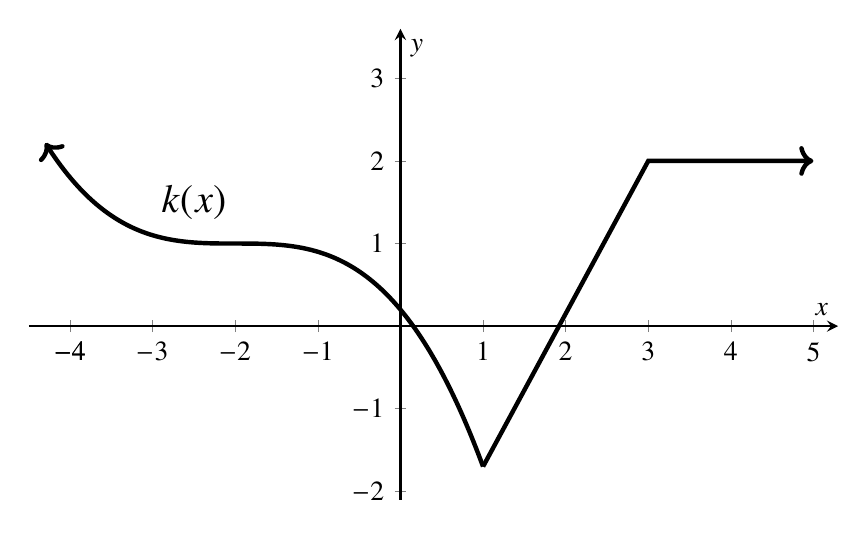
\begin{tikzpicture}[scale = 1]
\begin{axis}[scale=1.5, thick, my style, xtick={-4,-5,-4,...,5}, ytick={-2, -1,1,2,...,3},
xmin=-4.5, xmax=5.3, ymin=-2.1, ymax=3.6, minor y tick num=0,
        minor x tick num=0, mark size=3.0pt, grid=none, %both, %grid style={ thin, black, %dashed}, 
        axis equal image]
%\addplot[<-,ultra thick, smooth, variable=\x, samples=100, domain=-4:1] plot(\x,{-((-0.1)*(\x +2)^3-1)}); 
\addplot[<-,ultra thick, smooth, variable=\x, samples=100, domain=-4.3:1] plot(\x,{((-0.1)*(\x +2)^3)+1});    
\addplot[ultra thick, , ->] coordinates {(1, -1.7) (3,2) (5,2)};
\path (-2.5,1.5) node {\Large{$k(x)$}};
\end{axis}

\end{tikzpicture}

\bigskip

\begin{tikzpicture}[scale = 1]
\begin{axis}[scale=1.5, thick, my style, xtick={-4,-5,-4,...,5}, ytick={0},
xmin=-4.5, xmax=5.3, ymin=-3.6, ymax=3.6, 
        minor x tick num=0, mark size=3.0pt, grid=none,         axis equal image]

\end{axis}

\end{tikzpicture}

\end{center}


\newpage



\newpage




%%%%%%%%%% velocity and stuff


\problem{12 points} The position function $s(t)=8t-t^3$ gives the position in miles of a freight train running along a straight east-west railroad track where east is the positive direction and $t$ is measured in hours. Assume $t\geq 0.$
	\begin{subproblems}
	\item Find expressions for velocity and acceleration of the train at time $t.$
	
	%\textcolor{red}{2 points}
	\vfill
	\item What is the \emph{average} velocity of the train in the first two hours from $t=0$ to $t=2$? Include units.
	
	%\textcolor{red}{3 points}
	\vfill
	\item Determine the direction the train is traveling at the start of the trip when $t=0.$
	
	%\textcolor{red}{2 points}
	\vfill
	\item At $t=1,$ is the train speeding up or slowing down? Justify your answer.
	
	%\textcolor{red}{3 points}
	\vfill
	\item Determine the time (or times) at which the train changes direction or explain why this does not happen.
	
	%\textcolor{red}{2 points}
	\vfill
\end{subproblems}

\newpage

%\end{enumerate}
%%%%%%%%%%%%%%%%%%%%%%%%%%%

%\fbox{Extra Credit} 
\problem{Extra Credit: 5 points} %Consider the function $\displaystyle f(x)=\frac{2^x}{1-x}$.\\
\begin{subproblems}
\item On the given set of axes, draw a function $f(x)$ that satisfies all of the following properties. Label important points on the $x$- and $y$-axes. 
\begin{enumerate}[(i)]
\item $f(0)=2$
\item $f(5) = -2$
\item The domain of $f$ is the entire interval $[0,5].$
\item The graph of $f(x)$ never crosses the $x$-axis.
\end{enumerate}

\begin{tikzpicture}
\draw[<->] (-1, 0) -- (5,0);
\draw[<->] (0,5) -- (0,-5);
\end{tikzpicture}


\item The Intermediate Value Theorem says 
\begin{quote}
Let $f$ be continuous over a closed, bounded interval $[a,b]$.
 If $z$ is any real number between $f(a)$ and $f(b)$,
then there is a number $c$ in $[a,b]$ satisfying $f(c)=z$.
\end{quote}

Does your function contradict the statement of the Intermediate Value Theorem (IVT) or does it agree with the statement of the IVT?

If it contradicts the statement of the IVT, explain how. If it agrees with the statement of the IVT, explain how.


\vfill
\end{subproblems}

\end{document}

%%%%ENDDOCUMENT


